%% EPJ Data Science, Regular Article. Springer Nature LaTeX template v3.1 (sn-jnl), numbered references.
%% Draft compiled with Tectonic (XeTeX); source kept pdfLaTeX-compatible for submission (single file, no fontspec).
\documentclass[pdflatex,sn-mathphys-num,referee]{sn-jnl}

\usepackage{graphicx}
\usepackage{amsmath,amssymb}
\usepackage{booktabs}
\usepackage{xcolor}
\usepackage{tabularx}
\usepackage{array}
\usepackage[mathlines]{lineno}
\renewcommand{\linenumberfont}{\normalfont\tiny}
\usepackage{placeins}
\geometry{textwidth=170mm,textheight=230mm}
\AtBeginDocument{\setlength{\bibsep}{0.5em}}
\clubpenalty=10000
\widowpenalty=10000
\usepackage{url}
\graphicspath{{../figures/out/}}


\raggedbottom

\begin{document}

\title[Roots or beaches?]{Roots or beaches? Historical internal migration and holiday mobility in Spain}

\author*{\fnm{Alejandro} \sur{Treny Ortega}}\email{alejandro.ortega.26@ucl.ac.uk}

\affil*{\orgname{University College London}, \orgaddress{\city{London}, \country{United Kingdom}}}

\abstract{Does the geography of Spain's rural exodus still show up in where people spend their holidays? I link mobile-phone estimates of overnight stays across 2,435 mainland zones on 1,275 nights from 2022 to 2025 to census counts of city residents by province of birth. For each night I compare cities from the same province sending people to the same destination province, accounting for distance and income. On ordinary weekday nights in 2022--2024, the elasticity of overnight flows with respect to the birthplace share averages 0.52. In the held-out 2025 comparison of five August nights with 62 ordinary nights, the elasticity is higher by 0.134 (95\% confidence interval 0.037--0.233). In separate models the August increase is associated with the shares of residents who arrived in their province before 1981 and those born in municipalities of up to 2,000 people. The term for arrivals in 2016--2023 falls in 2022--2024 and has the same sign in 2025. On each of the 27 mid-August nights in 2022--2024, 97--99\% of the most depopulated zones receive more visitors than they send residents away. The flows describe all travellers from each city. The estimates show when overnight mobility aligns most closely with historical birthplace ties.}

\keywords{human mobility, mobile phone data, internal migration, holidays, gravity model, pre-registration, rural depopulation}

\maketitle
\linenumbers

%% ============================================================
\section{Introduction}\label{sec:intro}

On 13--14 February 2024, about 2.1 million mainland residents slept in a mainland zone other than their own. On 14--15 August, 8.5 million did. Groups of at least ten Madrid residents slept in 2,203 of the other 2,434 mainland zones that August night, compared with 1,124 in February. These trips take place against the backdrop of Spain's mid-twentieth-century rural exodus, when many people moved from the interior towards Madrid, Catalonia and the Basque Country \cite{clar2023rural,bover1999migrations,collantes2011peaceful}. The phrase \emph{volver al pueblo}, going back to the village, describes a familiar form of travel in Spain \cite{garciagonzalez2024retorno}.

An inland village may receive people who have family there, as well as hikers or visitors staying near a lake. The children and grandchildren of the rural migrants may have kept ties to the village, or may spend their holidays elsewhere. Visitor counts alone leave these explanations open. I ask whether the provinces a city sends its overnight visitors to are also the provinces where more of its residents were born.

Mobile-phone data make seasonal changes in population and mobility visible at national scale \cite{deville2014dynamic,silm2010seasonal,batistaesilva2020uncovering,blondel2015survey}. Wen and colleagues compare regular and holiday intercity networks in China and find that the correlates of travel change \cite{wen2026reframing}. He and colleagues compare mobility within Nanjing across two Spring Festivals \cite{he2026spatiotemporal}. Studies of homecoming periods also show differences in how travel varies with distance \cite{luan2024different,zhao2025effective}. Li and colleagues compare Spring Festival travel with a census migration matrix across 31 Chinese provinces using matrix correlations \cite{li2016spring}. I extend this kind of comparison to an ordinary-night baseline, city-to-province flows with distance and province-pair controls, and census measures that distinguish earlier and more recent arrivals.

In Spain, Garc\'ia-Gonz\'alez and colleagues use phone-based counts to describe return tourism in Castilla-La Mancha \cite{garciagonzalez2024retorno}. Garz\'on-Paredes and Royo-Vela examine how heritage stock relates to temporary population redistribution on selected dates \cite{garzon2026heritage}. Social networks help account for the geography of individual movement and regional connectedness \cite{cho2011friendship,bailey2018social,bailey2020europe,prietocuriel2024diaspora}. Migrant stocks also predict tourism flows \cite{etzo2014migration,santanagallego2022tourism}. Here I compare how strongly overnight flows follow birthplace ties over the calendar, and which city-level cohort shares are associated with the change. I registered the tests after looking at part of the 2022--2024 data, then tested the August contrast on unseen nights in 2025.

Cities send relatively more overnight visitors to the provinces where more of their residents were born. This association strengthens on mid-August nights, especially in the terms for earlier arrivals and for people born in small municipalities. I also describe how the balance between arrivals and departures changes in the most depopulated parts of mainland Spain.

The Supplementary Information (Additional file 1) compares the changes in network structure on selected nights with degree-preserving rewiring. The main analysis uses the full flow weights to study which city-to-province links grow.

%% ============================================================
\section{Data}\label{sec:data}

Table~\ref{tab:data} lists the sources, what each measures and how I use it. Figure~\ref{fig:design} shows the study area, the comparison and the coverage of each source.

\begin{table}[!htbp]
\caption{\textbf{Data sources.} Units, coverage and role of each source in the analysis.}\label{tab:data}
\footnotesize
\begin{tabularx}{\textwidth}{@{}>{\raggedright\arraybackslash}p{3.4cm}>{\raggedright\arraybackslash}X>{\raggedright\arraybackslash}p{3.35cm}>{\raggedright\arraybackslash}p{2.6cm}@{}}
\toprule
Source & What it measures & Coverage & Role \\
\midrule
Ministry overnight stays \cite{mitms2024methodology,mitmaovernightfiles} & Residents of zone $i$ who sleep in zone $j$ on one night, estimated from one operator's phones and scaled to the population & 2\,435 mainland zones, 1\,079 valid nights in 2022--2024 and 196 in 2025 & Nightly flow outcome \\ \addlinespace[4pt]
Census, table 68545 \cite{ine2026table68545} & Residents of each large city by province of birth, 1 January 2024 & 137 mainland cities, birthplace shares for 47 mainland provinces & Roots share, pooled model \\ \addlinespace[4pt]
Census 10\% sample \cite{ine2025censo} & Province of birth, year of arrival in the province, size of the birth municipality & 675 municipalities with $>10\,000$ inhabitants & Roots shares by group \\ \addlinespace[4pt]
Historical census series \cite{ine2026intercensal} & Population of each municipality 1900--2021 & Mainland municipal series & Depopulation rank \\ \addlinespace[4pt]
Income \cite{ine2026adrh} and housing \cite{ine2023viviendas} & Net income per person (2024) and non-primary dwellings (2021) & Municipalities & Controls and sensitivity \\ \addlinespace[4pt]
INE phone tourism matrices \cite{ine2026turismomoviles,gonzalezolmos2024measuring} and ECEPOV 2021 \cite{ine2023ecepovmicro} & Monthly municipal trips (three operators) and survey-reported birthplaces of parents & July 2019--September 2026 (trips), 137 origin cities & Validation and supplementary analyses \\
\botrule
\end{tabularx}
\end{table}

\begin{figure}[!htbp]
\centering
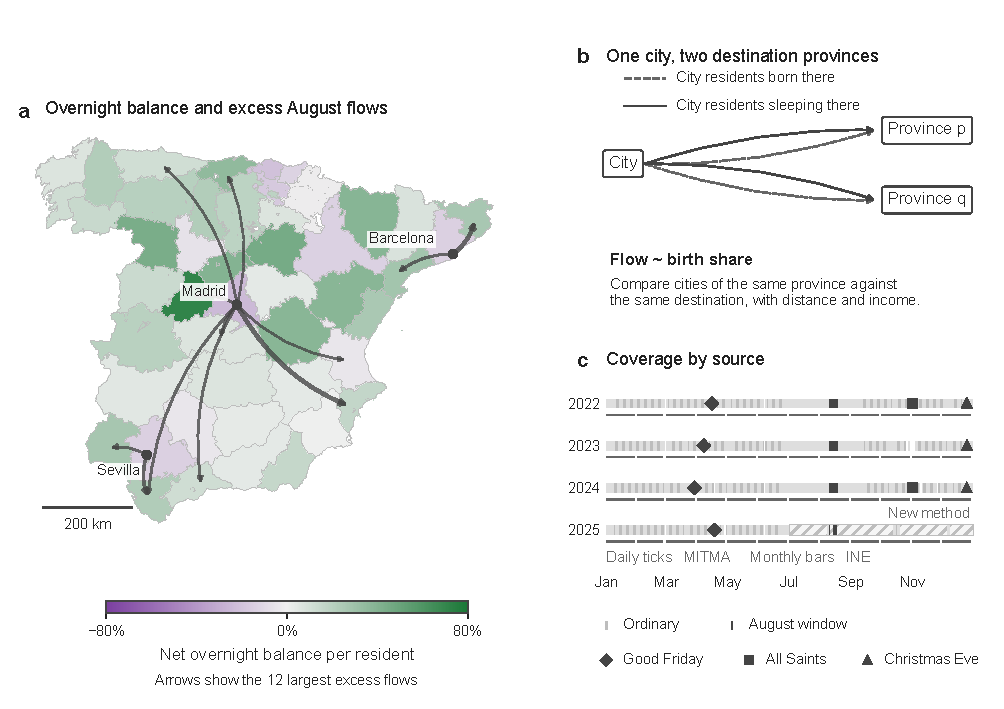
\includegraphics[width=\textwidth]{fig1.pdf}
\caption{\textbf{Linking overnight stays to birthplaces.} \textbf{a} Mainland provinces, shaded by net overnight stays per resident on 14--15 August 2024. Arrows connect cities to destination provinces. Their widths scale with the excess persons per night in the August window (nine nights ending on 10--18 August) over 92 ordinary nights in 2024, for the 12 largest excesses among 137 origin cities. \textbf{b} The model relates a city's overnight flow to the share of its residents born in the destination province, comparing cities within the same origin province and controlling for distance and income. \textbf{c} MITMA daily files and INE monthly files available from 2022 through 2025. Hatching marks the MITMA method introduced on 1 July 2025. Daily dates denote the morning at the end of the night.}
\label{fig:design}
\end{figure}

\subsection{Overnight stays}

The overnight estimates come from the Spanish transport ministry (MITMA in the figures) \cite{mitms2024methodology,mitmaovernightfiles,kotov2026spanishoddata}. Each phone of one operator is assigned a home zone, where it usually spends the night, and a zone for each observed night. The ministry expands the counts to the resident population. A zone is a municipality or a group of small neighbouring municipalities. The study frame covers 2,435 zones, 7,975 municipalities and 47 provinces on the mainland. A file dated $d$ holds the night ending on the morning of $d$, so the file dated 15 August covers 14--15 August. Of 1,096 calendar dates from 2022 to 2024, eleven files were missing, three available dates were on the ministry's incident list and three were within the Valencia flood exclusion. This left 1,079 nights. I also use the 196 available standard files for 2025.

On 1 July 2025 the ministry changed how it filters static devices \cite{mitms2025methodchange}. It recalculated six earlier dates. The mean absolute change in the pooled elasticity was 0.014, below the registered tolerance. Supplementary Section~S7 describes which terms were checked and how the two methods enter the 2025 comparison.

Single-operator estimates can be biased in ways that vary across places \cite{wesolowski2013impact,pappalardo2021evaluation,dennijs2026tale}. In six overlap months of 2024, the overnight totals between provinces correlate at $r=0.90$--$0.99$ with monthly overnight totals based on three operators from Spain's National Statistics Institute (INE). The comparison uses province-to-province person-nights (INE table 52997 \cite{ine2026table52997}). Supplementary Section~S1 also reports agreement with the municipal trip tables.

\subsection{Where residents were born}

The census table of residents by province of birth \cite{ine2026table68545} covers 137 large cities of the mainland, each a zone of its own. Of these, 112 lie in the 22 provinces that contain at least two such cities, which is what the comparison needs. The 10\% census sample \cite{ine2025censo} adds three facts for each resident of the 675 municipalities with more than 10,000 inhabitants that form a zone of their own: province of birth, year of arrival in the current province, and the size of the birth municipality. I group residents by arrival, before 1981 or 2016--2023, and by birthplace, a municipality of up to 2,000 inhabitants or one of more than 10,000. Arrival before 1981 is a marker of the exodus generation, not a definition of it: it records arrival in the province, not in the city, and includes people who moved for other reasons. For brevity I call all 675 municipalities \emph{cities}, although many are towns.

\subsection{Depopulation and other variables}

For each zone I measure how much of its population it lost as one minus the ratio of its 2021 population to the largest population it had between 1900 and 1960 \cite{ine2026intercensal}. The 475 zones with the largest losses are a fifth of the 2,376 zones eligible for ranking. I call them the \emph{most depopulated} zones below. A zone is \emph{coastal} if it touches the sea. Income per person comes from the national income atlas \cite{ine2026adrh}. Distances are straight lines from each city to the population-weighted centre of the destination province.

%% ============================================================
\section{Methods}\label{sec:methods}

\subsection{The roots elasticity}

For the residents of city $c$ who sleep in a mainland zone of another province $p$ on night $t$, $y_{cpt}$, I fit a Poisson pseudo-maximum likelihood (PPML) model \cite{santossilva2006log,correia2020fast,weidner2021bias}:
\begin{equation}
\mathrm{E}[\,y_{cpt}\,] = \exp\!\big(\beta_t \log s_{cp} + \alpha_{ct} + \gamma_{o(c)pt} + f_t(d_{cp}) + \lambda_{pt}\log \mathrm{inc}_c\big),
\label{eq:ppml}
\end{equation}
where $s_{cp}$ is the share of the city's residents born in $p$, $\alpha_{ct}$ a term for each city (how much its residents travel at all that night), $\gamma_{o(c)pt}$ a term for each pair of origin province $o(c)$ and destination province $p$, $f_t$ a quadratic in log distance, and $\lambda_{pt}$ lets income matter differently for each destination. PPML can include zero outcomes. I use the published flow weights, including weights below ten, and exclude flows within the city's province.

The province-pair term absorbs shared factors, such as the destination's overall popularity on that night. The model also accounts for each city's overall departures and its distance to the destination. Remaining city-specific ties, such as transport connections or home ownership, can still be associated with birthplace shares. I call $\beta_t$ the \emph{roots elasticity}. Holding the model terms fixed, a doubling of the share born in $p$ corresponds to $2^{\beta_t}$ times the expected number of overnight visitors from the city to $p$. The outcome counts all residents of the city who sleep anywhere in $p$.

To see which birthplace ties gain weight in August, I enter two group-specific shares together in the 675-city sample. One model compares arrivals before 1981 and in 2016--2023. The other compares people born in municipalities of up to 2,000 inhabitants and those born in municipalities of more than 10,000. Each share divides the group count for that city--province pair by the city's total census sample. I add 0.5 to each group count before taking logs. The sign of the pre-1981 and village-born contrasts is stable across alternative rules, but the size depends on the rule (Supplementary Section~S4).

\subsection{Holiday contrasts}

A holiday premium is a difference between nights. I classify every night by its evening. The \emph{August window} is the nine nights ending on 10--18 August, around the national holiday of 15 August. \emph{Ordinary nights} are Monday, Tuesday and Wednesday evenings that are not a public holiday, nor the day before or after one, in the country or in any of the five regions of Madrid, Catalonia, Andalusia, Valencia and the Basque Country. I also exclude 24 June--10 September, 20 December--7 January and Holy Week, from the Friday before Palm Sunday to Easter Monday. Holidays come from the \emph{Boletín Oficial del Estado} (BOE) \cite{boe2022calendar,boe2023calendar,boe2024calendar,boe2025calendar}. The secondary tests use Christmas Eve (24--25 December), the night ending on Good Friday (beginning on Holy Thursday), and the night ending on All Saints' Day (31 October--1 November).

I estimate the premium by fitting the holiday and ordinary nights of the same year together. Every control and fixed effect in Eq.~\eqref{eq:ppml} varies by night. A common roots slope and a roots-by-holiday term capture the contrast. The coefficient $\delta$ of the latter term is the change in elasticity, averaged with equal weight across years. As a diagnostic I compare each rolling window of nine consecutive \emph{eligible} ordinary nights with the remaining ordinary nights of the same year. The windows overlap and serve as a descriptive check.

\subsection{Inference}

Cities of the same province share unobserved influences, and the same cities appear on every night. I therefore cluster by origin province jointly across all stacked nights (22 clusters for the 112 cities, 44 for the 675) and compute two-sided $p$-values and pointwise 95\% confidence intervals with the wild cluster restricted score bootstrap \cite{kline2012score,webb2023reworking}, using Webb weights and 9,999 draws. I adjust the primary and secondary $p$-values separately using Holm's method. The intervals describe uncertainty across origin provinces for the observed nights.

\subsection{Pre-registration, confirmation and hold-out}\label{sec:prereg}

An earlier version had examined 306 nights. Before opening the other 779 available files from 2022--2024, I committed the night classes, quality rules, models, hypotheses, inference and decision rule on 27 November 2026. The primary tests were an increase in the pooled elasticity in August (P1), an increase in the pre-1981 arrival term (P2), and a larger increase for inland destinations than for coastal ones (P3). P3 compares inland and coastal flows on common city--province support. The secondary tests cover the three other holidays, the village-born and recent-arrival terms, and the difference between pre-1981 and recent arrivals.

All 27 August-window nights of 2022--2024 had already been examined. I recorded this as Deviation 1. The first August comparison therefore uses previously observed August nights and new ordinary nights. Before downloading any 2025 file, I registered a second comparison using five unseen August nights (ending on 10 and 14--17 August) and 62 unseen ordinary nights. An August claim qualifies for the abstract if it passes Holm correction in the predicted direction in either comparison and has the same sign in both. The first 2022--2024 fits kept three destination zones with data drop-outs that the design excluded (Deviation 2); I re-ran every 2022--2024 test without them, which changed no estimate by more than 0.0004 and no decision, and all values reported here come from that rerun (Supplementary Section~S8).

\subsection{The receiving end}

A zone is a \emph{net receiver} on a night when more people from elsewhere sleep in it than its own residents sleep elsewhere, counting all flows. For the most depopulated fifth of zones I compute, on every valid 2022--2024 night, the share of net receivers and, per resident, arrivals (visitors sleeping in the zone) and departures (residents sleeping elsewhere).

\subsection{Supplementary analyses}

Supplementary Section~S2 compares selected nights with degree-preserving null models \cite{maslov2002specificity,zhou2007structural,zhou2017second,vanwijk2010comparing,krings2012effects,cimini2019statistical}. Supplementary Section~S6 documents an exploratory comparison of survey-reported parental birthplaces with monthly municipal trips \cite{ine2023ecepovmicro,ine2026turismomoviles}, including the release threshold that limited the comparison.

%% ============================================================
\section{Results}\label{sec:results}

\subsection{Flows follow birthplaces every night}

The point estimate of the pooled roots elasticity is positive on all 1,275 nights (Fig.~\ref{fig:calendar}a). On the ordinary weekday nights of 2022--2024 it averages 0.521. A doubling of the share born in the destination province corresponds to about 43\% more expected overnight visitors at that elasticity, holding the model terms fixed.

In 2022--2024 the elasticity averages about 0.57 on Friday and Saturday evenings, 0.59 on Sundays and 0.60 in July. It averages 0.635 in the August window and 0.645 on the nights beginning on 18--31 August. For Christmas Eve, All Saints, the night ending on Good Friday and Epiphany eve, the means are 0.62, 0.60, 0.57 and 0.65. Some of the highest estimates come near the end of the summer holidays, after the peak in travel volume. On 30--31 August 2022, for example, the elasticity reaches 0.70.

\begin{figure}[!htbp]
\centering
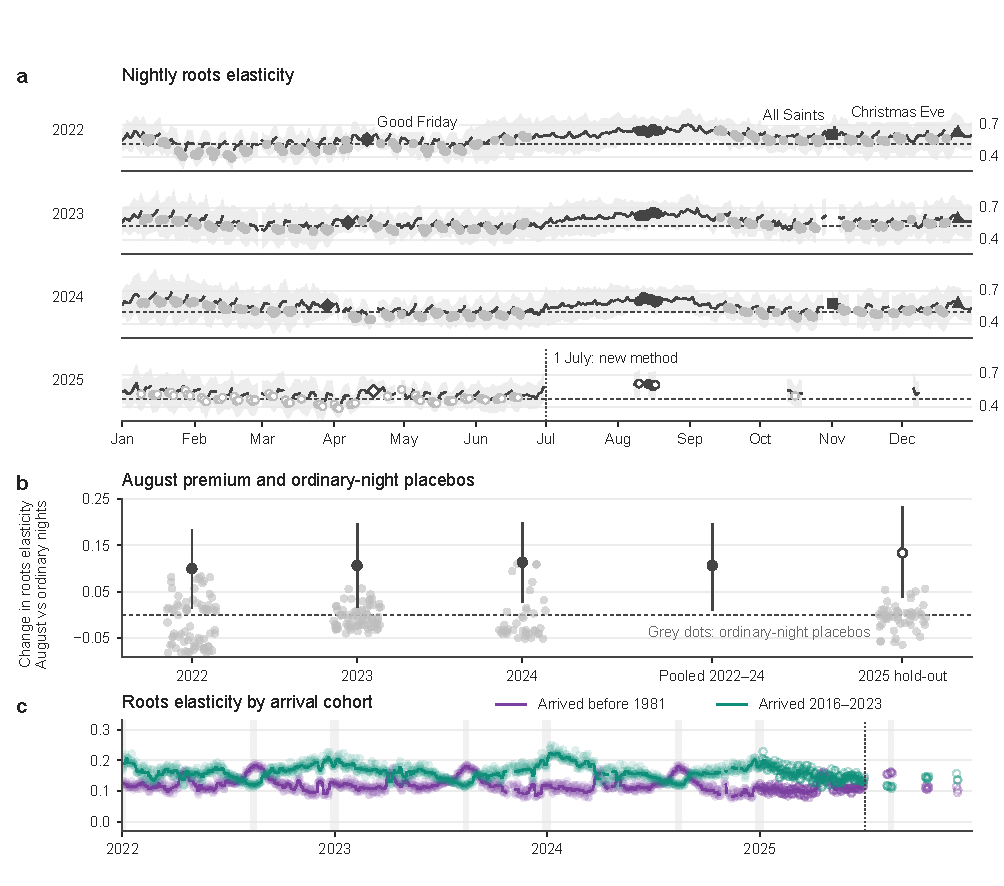
\includegraphics[width=\textwidth]{fig2.pdf}
\caption{\textbf{The roots calendar.} \textbf{a} Nightly roots elasticity for 112 cities in 22 origin provinces, with 95\% origin-province-clustered confidence ribbons. Open points show the 2025 series, including nights outside the hold-out contrast. Dashed lines show each year's ordinary-night mean. Holiday symbols mark nights ending on Good Friday, All Saints' Day or Christmas morning. \textbf{b} August minus ordinary-night contrasts and overlapping nine-night ordinary placebo windows. The 2022--2024 tests use new ordinary nights and previously seen August nights. The 2025 hold-out uses five unseen August nights and 62 unseen ordinary nights. Each placebo window has nine eligible ordinary nights. Intervals are 95\% cluster-robust intervals for the separate 2022--2024 years and 95\% wild-cluster bootstrap intervals for pooled 2022--2024 and 2025. \textbf{c} Joint arrival-cohort terms for 675 cities. Lines show centred seven-night rolling medians within continuous coverage, with gaps at the method change. Grey bands mark August test dates and Christmas Eve through Epiphany eve. Open markers mark 2025.}
\label{fig:calendar}
\end{figure}

\subsection{The August premium}

Table~\ref{tab:tests} gives the pre-registered tests. Supplementary Section~S8 reports the discovery and all-night comparisons. Against new ordinary nights of 2022--2024, the August elasticity is higher by 0.106 (95\% CI 0.010--0.197). The increase is similar in each year (0.10, 0.11 and 0.11) and larger than every one of the 188 nine-night placebo windows of ordinary nights (Fig.~\ref{fig:calendar}b), but after Holm correction its $p$-value is 0.067, so P1 did not pass the adjusted threshold in 2022--2024. In the 2025 hold-out, where both the August nights and the ordinary nights were unseen, the premium is 0.134 (95\% CI 0.037--0.233; Holm $p=0.030$), and it is again above all 54 placebo windows. The 2025 placebo windows contain nine nights each, while the August window has five observations. Measuring roots with the 2025 census instead of the 2024 one gives 0.131. The pooled August contrast meets the registered decision rule through the 2025 result.

At the 2025 estimate of 0.134, the flow ratio associated with doubling the birthplace share is about 10\% higher in August than on ordinary nights ($2^{0.134}\simeq1.10$). Across the 2022--2024 robustness checks the pooled estimate ranges from 0.07 to 0.15, with intervals that cross zero when using road travel time ($p=0.069$) or giving each night equal weight ($p=0.060$). These robustness $p$-values are unadjusted (Supplementary Section~S3).

\begin{table}[!htbp]
\caption{\textbf{Pre-registered tests.}}\label{tab:tests}
\footnotesize
\setlength{\tabcolsep}{3pt}
\begin{tabular*}{\textwidth}{@{\extracolsep\fill}lrlrlrlc}
\toprule
 & \multicolumn{3}{c}{2022--24} & \multicolumn{3}{c}{2025 hold-out} & \\
\cmidrule{2-4}\cmidrule{5-7}
Hypothesis & Est. & 95\% CI & $p$ & Est. & 95\% CI & $p$ & Conf. \\
\midrule
P1 August, all residents & $+0.106$ & [$0.010$, $0.197$] & 0.067 & $+0.134$ & [$0.037$, $0.233$] & 0.030 & yes \\
P2 August, arrived before 1981 & $+0.071$ & [$0.041$, $0.092$] & $<$0.001 & $+0.057$ & [$0.022$, $0.076$] & 0.010 & yes \\
P3 August, inland minus coast & $+0.122$ & [$-0.037$, $0.280$] & 0.11 & $+0.129$ & [$-0.055$, $0.319$] & 0.14 & no \\
\midrule
S1 Christmas Eve & $+0.088$ & [$0.049$, $0.177$] & $<$0.001 & --- & & & yes$^{a}$ \\
S2 Good Friday & $+0.037$ & [$-0.041$, $0.110$] & 0.25 & $+0.076$ & [$-0.013$, $0.157$] & 0.15 & no \\
S3 All Saints & $+0.073$ & [$0.022$, $0.135$] & 0.017 & --- & & & yes$^{a}$ \\
S4 August, born in a village & $+0.073$ & [$0.055$, $0.095$] & $<$0.001 & $+0.056$ & [$0.031$, $0.078$] & 0.004 & yes \\
S5 August, arrived 2016--2023 & $-0.044$ & [$-0.070$, $-0.011$] & 0.017 & $-0.033$ & [$-0.060$, $0.006$] & 0.15 & yes \\
S6 August, pre-1981 minus recent & $+0.115$ & [$0.071$, $0.139$] & $<$0.001 & $+0.089$ & [$0.034$, $0.117$] & 0.004 & yes \\
\botrule
\end{tabular*}
\footnotetext{Change in the roots elasticity relative to ordinary weekday nights of the same year. August contrasts use 27 previously seen August nights and 212 new ordinary nights in 2022--2024, and 5 unseen August nights and 62 unseen ordinary nights in 2025. Intervals are pointwise 95\% wild-cluster bootstrap intervals. The $p$-values are Holm-adjusted within each family. The final column gives the combined August decision or the secondary result for the periods available.}
\footnotetext{$^{a}$ Secondary results from 2022--2024 only (Christmas Eve, 3 holiday and 212 ordinary nights. All Saints, 2 holiday and 131 ordinary nights).}
\end{table}

\subsection{August contrasts by arrival cohort and birthplace size}

When the two arrival shares enter together, the pre-1981 term increases by 0.071 (95\% CI 0.041--0.092) in 2022--2024 and by 0.057 (0.022--0.076) in 2025. The recent-arrival term falls by 0.044 and 0.033, with an interval that crosses zero in 2025. In the birthplace-size model, the village-born term rises by 0.073 and 0.056 (Table~\ref{tab:tests} and Fig.~\ref{fig:who}a). In the 2022--2024 nightly series, the pre-1981 term averages 0.18 on August-window nights and 0.10 on ordinary nights. The recent-arrival term is lowest in August (0.12--0.13) and highest around Christmas, New Year and Epiphany (about 0.20--0.22, Fig.~\ref{fig:calendar}c). Both models use overnight stays by all residents of the city.

\begin{figure}[!htbp]
\centering
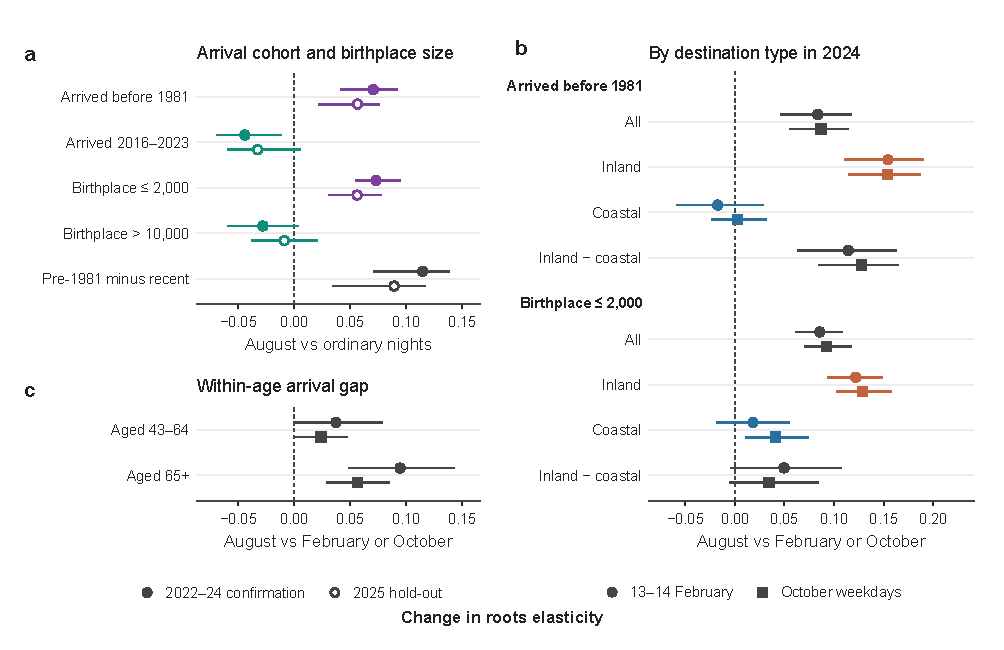
\includegraphics[width=\textwidth]{fig3.pdf}
\caption{\textbf{Which birthplaces gain weight in August.} All horizontal axes show changes in roots elasticity. \textbf{a} Arrival-cohort and birthplace-size contrasts for 675 cities across 44 origin provinces. Filled points show 2022--2024 confirmation against new ordinary nights. Open points show the 2025 hold-out. The urban-born contrast is the companion term of the village-born model. \textbf{b} Contrasts for 14--15 August 2024 against 13--14 February (circles) and the mean of 12 October weekday nights (squares); the first row of each panel labels the symbols. Inland and coastal labels refer to destination zones. The direct difference uses the 19 provinces with both types of destination. \textbf{c} Pre-1981 minus later-arrival contrasts for the same nights within two age bands. The later group is 2016--2023 arrivals for ages 43--64 and arrivals from 1981 onwards for ages 65 and over. All intervals use origin-province clusters. The urban-born row shows 95\% cluster-robust intervals. The other rows use 95\% wild-cluster bootstrap intervals.}
\label{fig:who}
\end{figure}

The gap is also visible within age bands in the 2024 comparisons. Among residents aged 65 and over, the August increase in the term for people who arrived before 1981 exceeds the increase for later arrivals by 0.095 against February and 0.057 against October. Among those aged 43--64 the comparator is arrivals in 2016--2023, with gaps of 0.040 and 0.034 (Fig.~\ref{fig:who}c). The pre-1981 and village-born contrasts remain positive without Madrid and Barcelona, in the 44 origin-province omissions, and in all 117 overlapping August--February night pairs. The pre-1981 coefficient ranges from 0.014 to 0.122 across zero-cell rules (Supplementary Section~S4).

\subsection{Inland destinations and other holidays}

In the 2022--2024 comparison the estimated premium is concentrated inland. The inland-only estimate is 0.138 (95\% CI 0.024--0.223) and the coastal-only estimate is 0.011 ($-0.135$ to 0.134). The direct test of a larger inland premium (P3) misses the adjusted threshold in both periods. The 2022--2024 difference is 0.001 after omitting Madrid and Barcelona as origins. The separate 2024 cohort analysis compares the same 19 provinces with both destination types. For the pre-1981 term it gives inland-minus-coastal differences of 0.114 against February and 0.128 against October (Fig.~\ref{fig:who}b).

In 2022--2024 the estimated premium is 0.088 (95\% CI 0.049--0.177) on Christmas Eve and 0.073 (0.022--0.135) on the night ending on All Saints' Day. Neither holiday has a 2025 observation. The Good Friday contrast is not detected in either period.

\subsection{The receiving end}

\begin{figure}[!htbp]
\centering
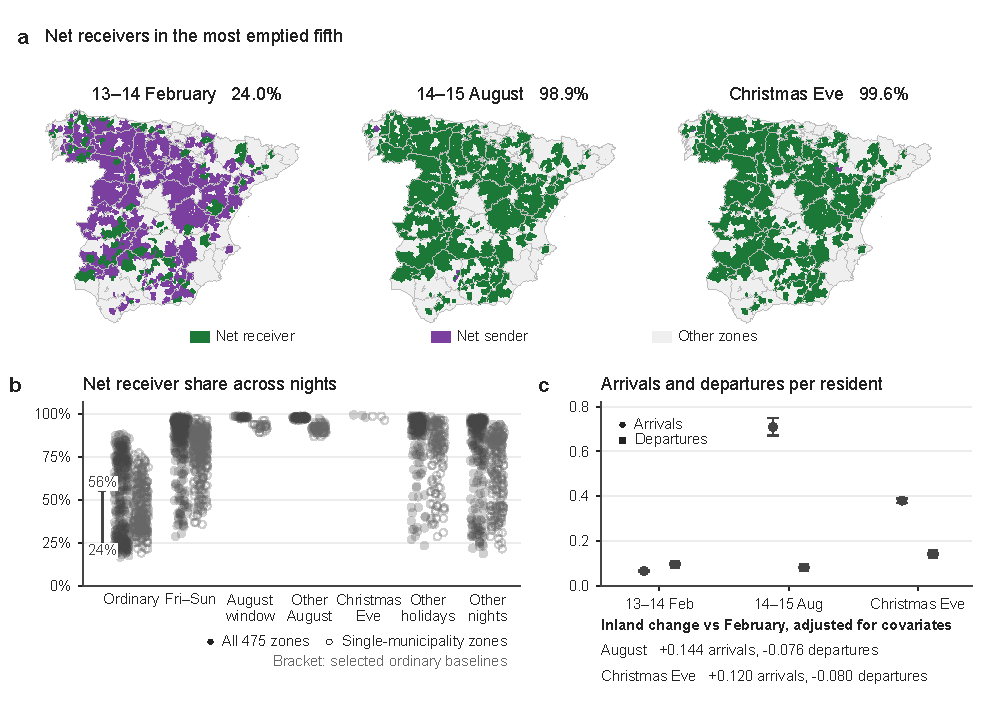
\includegraphics[width=\textwidth]{fig4.pdf}
\caption{\textbf{The receiving end of holiday mobility.} \textbf{a} Zones in the most emptied fifth (475 of 2,376 zones ranked by population loss from their 1900--1960 peak), coloured by net overnight balance on three nights in 2024. \textbf{b} Share receiving more people than they send on each of 1,079 valid nights in 2022--2024, by type of night, for all 475 zones (filled) and for the 84 comprising a single municipality (open); ordinary weekday nights are split by season (evening dates). \textbf{c} Mean arrivals (visitors sleeping in the zone) and departures (residents sleeping elsewhere) per resident in the most emptied fifth, with values and 95\% within-province zone-bootstrap intervals. The table below the panel gives adjusted changes per unit of population-loss rank in 2,053 inland zones.}
\label{fig:receiving}
\end{figure}

On ordinary weekday nights from November to March, monthly mean net-receiver shares in the most depopulated fifth range from 27\% to 39\%. From April to June and in September they range from 72\% to 82\%. On the 27 August-window nights of 2022--2024 the share is 97--99\%, and on Christmas Eve 2024 it is 99.6\% (Fig.~\ref{fig:receiving}). On 14--15 August 2024 the mean was 0.71 visitors per resident, compared with 0.07 on 13--14 February. Departures per resident moved from 0.10 to 0.08. Among inland zones the adjusted association between historical population loss and the August change in net balance is about two thirds more arrivals and one third fewer departures (Supplementary Section~S5).

\subsection{Municipal trip counts}

The municipal trip tables cannot establish whether August trip counts rise for villages where residents' parents were born. The result depends on how unpublished small flows are treated (Supplementary Section~S6).

%% ============================================================
\FloatBarrier
\section{Discussion}\label{sec:discussion}

The August nights show a stronger association between overnight stays and birthplace ties than ordinary weekdays in the held-out year. The cohort contrasts show which city-level birthplace shares gain weight: earlier arrivals and people born in smaller municipalities. The direct comparison leaves the size and sign of the inland--coastal difference uncertain. The analysis leaves room for other reasons to travel to the same places.

Models of spatial interaction typically account for population and distance \cite{simini2012universal,lenormand2016systematic,barbosa2018human}. Studies of migration and tourism add migrant stocks and social ties \cite{etzo2014migration,santanagallego2022tourism,bailey2018social,janta2015rethinking}. The overnight calendar shows how the latter association changes across dates and cohort definitions. The results add a birthplace comparison to earlier accounts of temporary population in inland Spain \cite{garciagonzalez2024retorno,delgadourrecho2014importancia}. Holding degree sequences fixed reproduces most of the observed change in degree assortativity (Supplementary Section~S2).

Population registers describe where people usually live. Overnight flows add a measure of how many people are present at particular times, including visits outside registered accommodation \cite{back2017mapping,vinuesa2005poblacion,garciagonzalez2024retorno}. The seasonal shifts in net balance can inform planning for services that respond to the population present.

\subsection{Limitations} The census and flow records cannot identify individual travellers, their reasons for travelling or their accommodation. The slope uses cities large enough for the census tables and comparisons within origin provinces that have multiple such cities. Year of arrival refers to the current province. The pre-1981 term can capture ties formed for reasons other than the rural exodus. The main exposure is measured in 2024, and the composition of cities may have changed over the study period. The hold-out contains five August nights measured with the new method and 62 ordinary nights, of which 61 use the old method. The six date pairs used to bridge the methods include no August night and cover two coefficients. Even if the method change had raised every August estimate by the largest shift seen on those dates, both confirmed August contrasts would stay above zero (Supplementary Section~S7). A measurement shift specific to summer, particular destinations or other cohorts remains possible. August is also compared with ordinary weekdays outside the main summer season, so the contrast combines holiday timing with season and day of week. The June and September sensitivity narrows the seasonal gap but cannot isolate a holiday effect.

\subsection{Outlook} Where both overnight flows and birthplace counts are available, the same model can compare their association across local holiday calendars. Surveys that ask travellers about family origins and trip purpose would address the individual question left open by the aggregate data.

%% ============================================================
\pdfbookmark[1]{List of abbreviations}{abbreviations}
\section*{List of abbreviations}
BOE, \emph{Boletín Oficial del Estado} (Spain's official gazette).
CI, confidence interval.
ECEPOV, \emph{Encuesta de Características Esenciales de la Población y las Viviendas}.
GISCO, Geographic Information System of the Commission.
INE, \emph{Instituto Nacional de Estadística}.
MITMA, Spanish transport ministry's mobility data source.
PPML, Poisson pseudo-maximum likelihood.

\backmatter

\section*{Supplementary information}\label{sec:si-file}
Additional file 1 (\nolinkurl{supplementary.pdf}, PDF) contains data validation, network diagnostics, robustness and cohort checks, the receiving-end decomposition, the parental-birthplace analysis, the 2025 method bridge and deviations from the pre-registration.

\section*{Declarations}

\subsection*{Availability of data and materials}
The Spanish transport ministry publishes the overnight-stay files \cite{mitmaovernightfiles}. Spain's National Statistics Institute provides the census tables and public-use microdata, historical municipal populations, income, housing and phone-based tourism matrices \cite{ine2026table68545,ine2025censo,ine2026intercensal,ine2026adrh,ine2023viviendas,ine2026turismomoviles,ine2023ecepovmicro}. Municipal boundaries for the supplementary parental analysis are from Eurostat's Geographic Information System of the Commission (GISCO) \cite{gisco2021lau}. The derived city--province tables, nightly estimates and every result needed to reproduce the tables and figures are distributed with the code (see Code availability).

\subsection*{Code availability}
Analysis code, the pre-registration and its deviations, and the derived data behind every table and figure are archived on Zenodo (\url{https://doi.org/10.5281/zenodo.24624569}). The code is also maintained at \url{https://github.com/aleetreny/spain-holiday-roots} (branch \texttt{journal}).

\subsection*{Competing interests}
The author declares no competing interests.

\subsection*{Funding}
This research received no specific funding.

\subsection*{Authors' contributions}
A.T.O. designed the study, analysed the data and wrote the manuscript.

\subsection*{Acknowledgements}
I thank Professor Shi Zhou (University College London), in whose Complex Networks module this work began, and the Spanish Ministry of Transport and Sustainable Mobility and the National Statistics Institute (INE) for publishing the data used here as open data.

\subsection*{Ethics approval and consent to participate}
Not applicable. The analysis uses only published aggregate statistics and public-use microdata released by public agencies. No participant was contacted and no individual mobility record was accessed.

\subsection*{Consent for publication}
Not applicable.

\subsection*{Use of AI tools}
The author used large language model assistants for help with the analysis code and the figures. The author designed the study, checked all code, results and text, and takes full responsibility for the content.

\bibliography{references}

\end{document}
